\chapter{Data Analysis}\label{chap:02}

\section{Experiment Setup}
The setup consists of a single fiber stretched from one end to the other and an LED mechanism that can move very close to and along the length of the fiber. At the end of the fiber is a rotating arm spectrometer that can register the light coming out of the fiber at various angles both vertical and horizontal, it can be tilted in the horizontal
and vertical plane within the angle intervals [-20°,90°] and [-6°,90°], respectively.
The simulation data is produced using Geant4 for a 50 fiber structure with excitations on 24 points across each fiber. No other details about Geant4 or production process of the simulation data is discussed.

\section{Measurements}
For every measurement, a dark count data where the measurements are taken while the LED is turned off is also taken. This will be integral in the analysis, where the dark count data will be subtracted from the actual counts to remove the background. The current of the LED is set to 20 mA for all measurements as well as the integration time which is set to $10000 \mu$s and number of averages which is set to 5 in all measurements.

\subsection{Spectrometer Measurement}
The first measurement is taken without giving any specific input into the machines to test the dependence of the system to the ambient light in the room. Two measurements are taken with the roomlight on and off.

\subsection{Radial symmetry Measurement}
This measurement is taken to test the radial symmetry of the spectrometer setup, the horizontal and vertical angle of the spectrometer are varied while the excitation position on the fiber from the LED is kept constant. The interval of angles used in this measurement is $\left[-18^{\circ}, 30^{\circ}\right]$ in the horizontal and $\left[-6^{\circ}, 35^{\circ}\right]$ in the vertical. 13 measurements are taken in both cases.

\subsection{Intensity Measurement}
For the last measurement, the intensity of light received at the spectrometer end depending on the distance is measured moving the LED structure on the axis of the fiber, hence moving the excitation point. The fiber is excited in a total range of 150 cm in 7.5 cm increments. For each excitation point, 10 different horizontal angles in the interval $\left[0^{\circ}, 40^{\circ}\right]$ are measured.

\section{Measurement Analysis}
\subsection{Spectrometer Measurement}
This section only relates to the emission spectrum of the LED we are using and the decision to turn off the roomlight before taking the consequent measurements. In \hyperref[Roomlight]{Figure 2.1}, the LED signal can be picked up more clearly for the measurements where we have the roomlight turned off.
\begin{figure}[h]
    \centering
    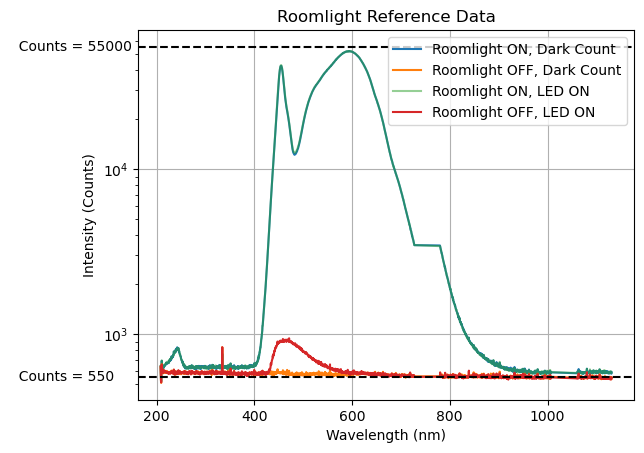
\includegraphics[width=0.7\linewidth]{graphs/Roomlight.png}
    \caption{Spectrometer Measurement with Roomlight and LED toggled.}
    \label{Roomlight}
\end{figure}

If we proceed to then subtract the dark count values where the LED is turned off from the counts where we had the LED turned on, we get the following \hyperref[Roomlight_corr]{Figure 2.2.}.

\begin{figure}[h]
    \centering
    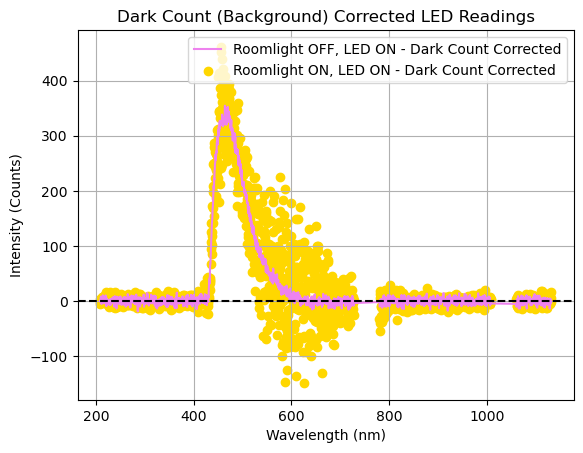
\includegraphics[width=0.7\linewidth]{graphs/Roomlight_corr.png}
    \caption{LED signal isolated graph by subtracting dark counts.}
    \label{Roomlight_corr}
\end{figure}

This makes the difference in the two datasets much more visible as the LED signal is smeared and has a lot of uncertainty for the dataset with the roomlight on. So the decision is made to turn off the roomlight while the rest of the measurements are taken.

\subsection{Radial symmetry Measurement}
Our 2-D histogram for total photon count plotted against varied angles of horizontal and vertical position of the spectrometer can be seen in the \hyperref[Radialsym]{Figure 2.3}. This result uses the dark counts subtracted version for dark counts taken at each position of the spectrometer. It shows that radially, there is a symmetry in our reading and for the rest of the measurements we can make the decision to utilize only the horizontal axis to take angular dependent measurements. This is because same amount of displacement in the vertical axis would give the same data as the horizontal axis.
\begin{figure}[H]
    \centering
    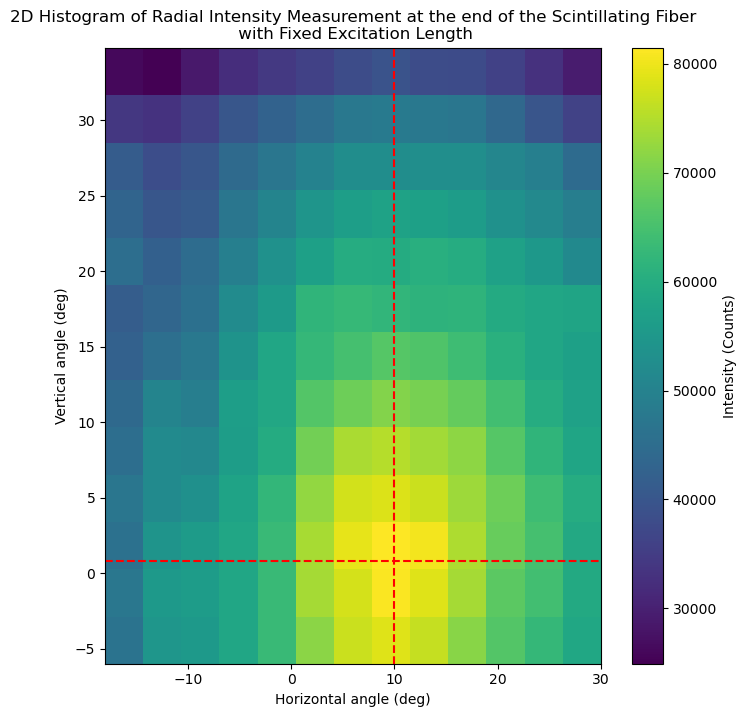
\includegraphics[width=0.7\linewidth]{graphs/radialsym.png}
    \caption{Measurement from the spectrometer angled at different points at the fiber end while the excitation point on the fiber is kept constant}
    \label{Radialsym}
\end{figure}
%\newpage <-- this command crashes the compiler

\subsection{Intensity Measurement}
The final measurement gives us the data for intensity at various angles at increasingly distant excitation points. The complete data is plotted in \hyperref[intensitymeasured]{Figure 2.4}. There are some obvious observations to be made such as the number of photons reaching the end of the fiber dropping as the excitation distance increases and the larger spectrometer angle measurements yielding less counts than those more inline with the fiber axis. The surprising observation here is the sudden drops of photon counts right after moving away from 100mm and 600mm excitation lengths. Our explanation for this is either a significant kink or imperfection in the fibre at those points or a disturbance of the experiment setup. We reason that these kinky regions are unrelated to our theory and to avoid them we produce decreasing power law fits for 3 intervals of excitation length without kinks: 0-75mm, 150-650mm and 725-1500mm. 

\begin{figure}[H]
    \centering
    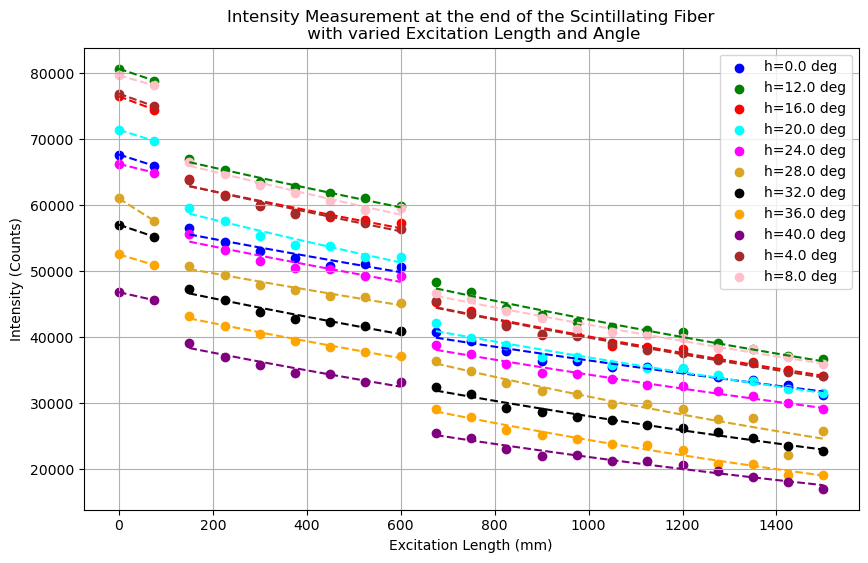
\includegraphics[width=0.8\linewidth]{graphs/Intensity_meas_fitted.png}
    \caption{Excitation Length and spectrometer angle dependent measurement of intensity at the end of the fibre}
    \label{intensitymeasured}
\end{figure}

\section{Simulation Analysis}

The simulation consists of a dataframe from the GEANT4 software with 12194 simulated data points, each having 15 features. They are simulations of photons propagating down the fiber and getting registered at the photomultiplier end with a given momentum, position and angle with respect to the fiber center axis as well as some valuable attributes.

\subsection{Un-physical photons}

There are events in this dataset where the point at which the photons are supposed to be registered fall outside the width of the excited fiber of 0.125mm. We consider these points as mistakes in the simulation and remove them before proceeding. The removal is done by calculating the exit position vector of the photon and removing all data point with an exit radius larger than 0.125mm as can be seen in \hyperref[unphysical]{Figure 2.5}

\begin{figure}[H]
    \centering
    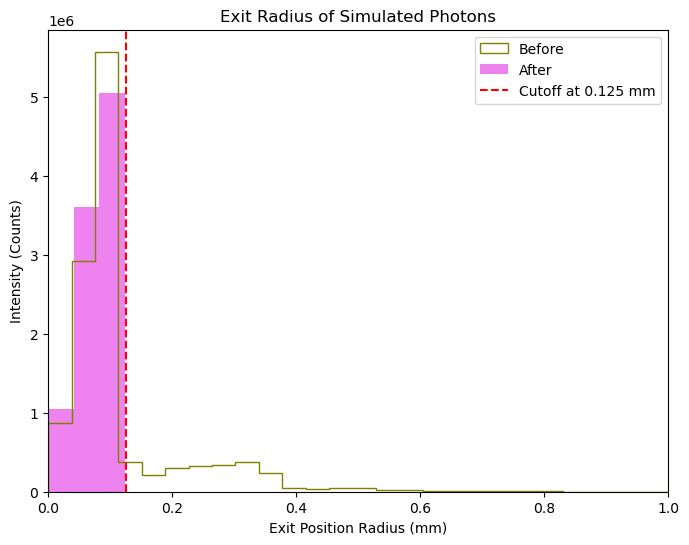
\includegraphics[width=0.7\linewidth]{graphs/unphysical.png}
    \caption{Removal of photons with exit coordinates that fall above the width of the scintillating fiber}
    \label{unphysical}
\end{figure}

Another attribute we can use for selecting physical events is to utilize the angle at which the photons arrive at the end of the scintillating fiber. From the internal structure of the fiber, we know that the maximum angles for which internal reflection occurs can be determined with the following forms of Snell's Law:


\begin{equation}
\begin{aligned}
& \theta_{1}=\arccos \left(\frac{n_{2}}{n_{1}}\right)=21.37^{\circ} \text { for core-cladding  and } \\
& \theta_{2}=\arccos \left(\frac{n_{3}}{n_{1}}\right)=27.44^{\circ} \text { for cladding-cladding reflected photons }
\end{aligned}
\end{equation}

Where n's denote the refractive indexes of the mediums as shown in \hyperref[Individual Fiber]{Figure 1.3}
Which means any photons incident on the fiber end with a higher angle must be unphysical as well. Another attribute of the simulation dataset is that it tags photons based on whether they are coming from a core-cladding or cladding-cladding interface reflection, therefore allowing us to separate the dataset into two and apply two seperate cuts based on the reflection origin of the photon as shown in \hyperref[reflunphys]{Figure 2.6}.

\begin{figure}[H]
    \centering
    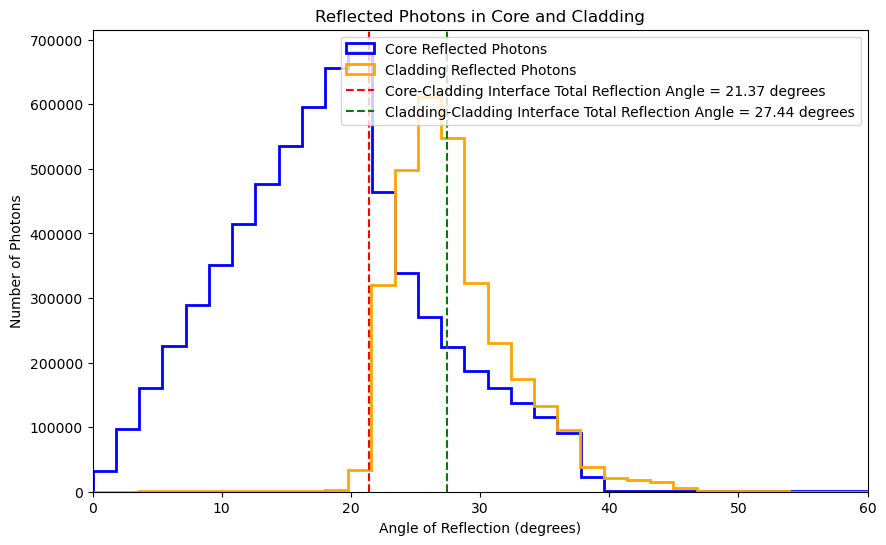
\includegraphics[width=1\linewidth]{graphs/unphysical_refl.png}
    \caption{Removal of photons with reflection angles higher than physically allowed}
    \label{reflunphys}
\end{figure}

\subsection{Minimum distance ($r_{min}$)}
The minimum distance between the path of the photon and the center of the fiber axis ($x$-axis), as seen in \hyperref[Scifi Diagram]{Figure 1.4}, is given by the formula:

\begin{equation}
r_{\min }=\left|\frac{z p_{y}-p_{z} y}{\sqrt{p_{z}^{2}+p_{y}^{2}}}\right|
\end{equation}

Where $y, z, p_{y}$, and $p_{z}$ are the positions and momenta of the photon at its creation point in the fiber. This formula is obtained by calculating the minimal distance of the photons path (starting point $x, y, z$ and direction $p_{x}, p_{y}, p_{z}$ ) from the $x$-axis. In order to visualize the connection between this quantity and the reflection angle, we can plot the following 2-D histograms for core-cladding and cladding-cladding photons respectively.

\begin{figure}[H]
    \centering
    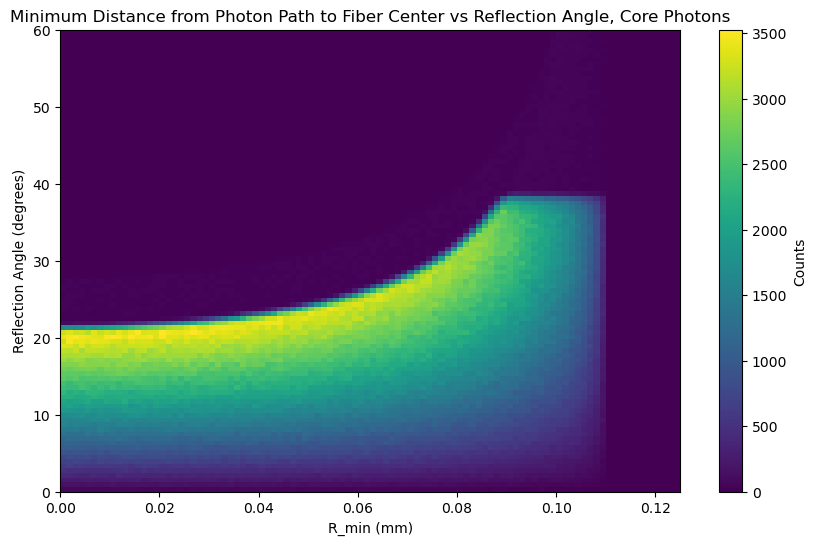
\includegraphics[width=0.75\linewidth]{graphs/corerefl.png}
    \caption{2-D histogram of reflection angle and $r_{min}$, for core photons}
    \label{corerefl}
\end{figure}

\begin{figure}[H]
    \centering
    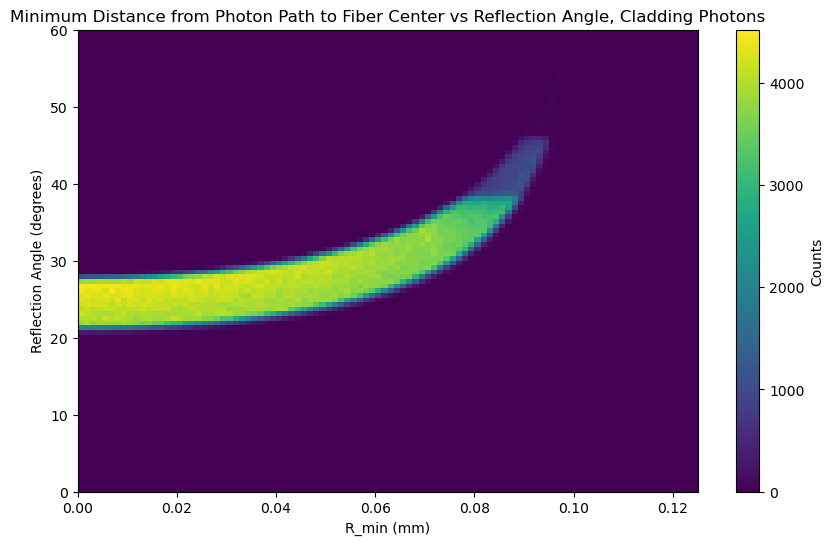
\includegraphics[width=0.75\linewidth]{graphs/cladrelf.png}
    \caption{2-D histogram of reflection angle and $r_{min}$, for cladding photons}
    \label{cladrefl}
\end{figure}

We can see that as the minimum distance from the centre of the fiber axis increases, the reflection angle is expected to be higher where the photon ends up following a helical trajectory down the fiber structure. Also of note is that any angle larger than the maximal angle will result in total reflection, hence the distribution seen in both histograms. The cladding photons specifically have to interact with 3 interfaces and hence are not retained below a certain reflection angle.

\subsection{Attenuation}
The final analysis to be done on the simulation data is to illustrate the attenuation, or the intensity of photons that reach the end of the fiber with varying reflection angles and excitation length. The following histogram shows the relation between the two parameters discussed in the intensity formula \hyperref[1.8]{Equation 1.8} for core-cladding and cladding-cladding photons respectively.

\begin{figure}[H]
    \centering
    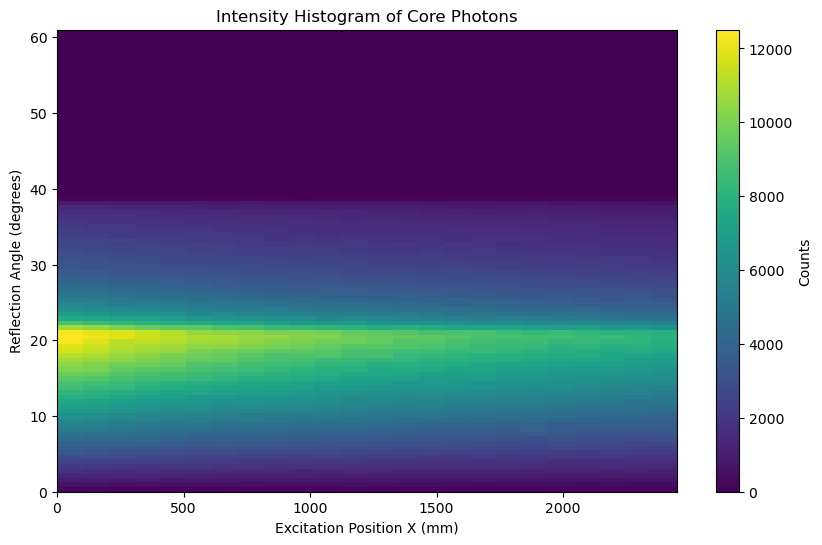
\includegraphics[width=0.65\linewidth]{graphs/coreint.png}
    \caption{Intensity of core-cladding interface reflected photons, plotted as a 2-D histogram with reflection angle and excitation position attributes}
    \label{fig:enter-label}
\end{figure}

\begin{figure}[H]
    \centering
    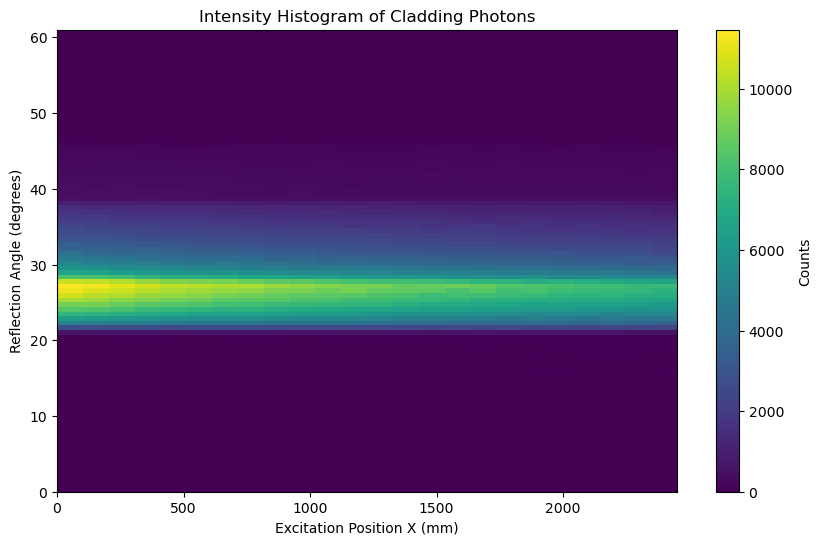
\includegraphics[width=0.65\linewidth]{graphs/cladint.png}
    \caption{Intensity of cladding-cladding interface reflected photons, plotted as a 2-D histogram with reflection angle and excitation position attributes}
    \label{fig:enter-label}
\end{figure}

Using the counts from the histogram bins, we performed curve fits of the intensity in relation to all the increments of excitation length. The intensity function used in the fits will be the following from \hyperref[1.3]{Section 1}:

\begin{equation}
I(x)=I_{0} \exp (-a L) \tag{1.3}
\end{equation}

\begin{figure}[h]
    \centering
    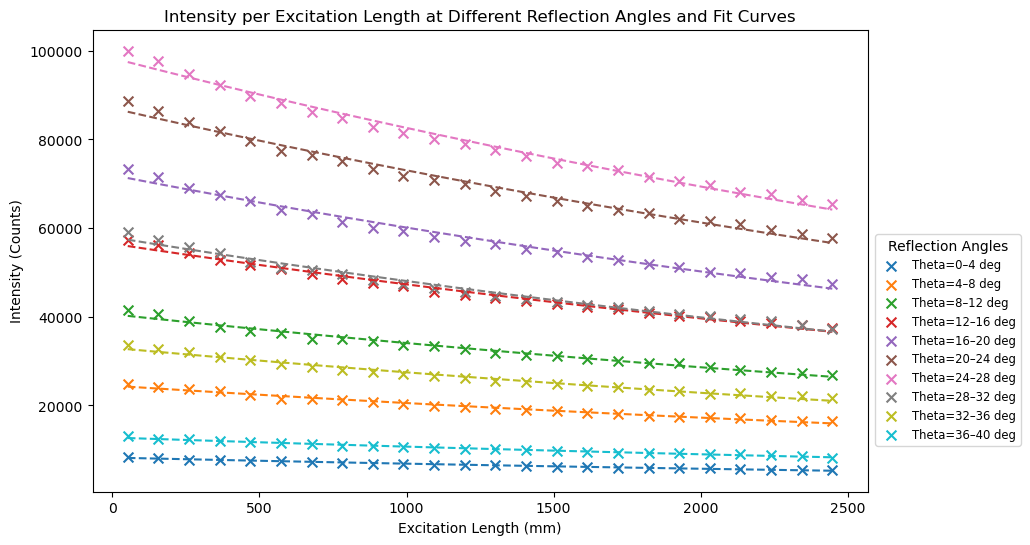
\includegraphics[width=1\linewidth]{graphs/exc_length.png}
    \caption{Simulation and curve fits for intensity at the end of the fiber for different reflection angles and excitation lengths}
    \label{exc}
\end{figure}

Moreover, we can compare the three different ways it is possible for us to acquire the $a_{eff}$ parameter and test our analysis accuracy. For the simulation analysis part, we are going to extract the term from the exponential decay fit in the \hyperref[exc]{Figure 2.11}. For a theoretical curve, we are going to average the parameters acquired from simulation analysis and make a continuous curve by fitting to the following equation:

\begin{equation}
a(\theta)=\frac{A}{\cos (\theta)}+B \tan (\theta), 
\end{equation}

And lastly, we are going to exponential decay fit our data points from the \hyperref[intensitymeasured]{Figure 2.4}, where the data comes from our measurement\cite{SciPy}. Plotting the results from the three approaches gives us the following parameter distribution:

\newpage

\begin{figure}[h]
    \centering
    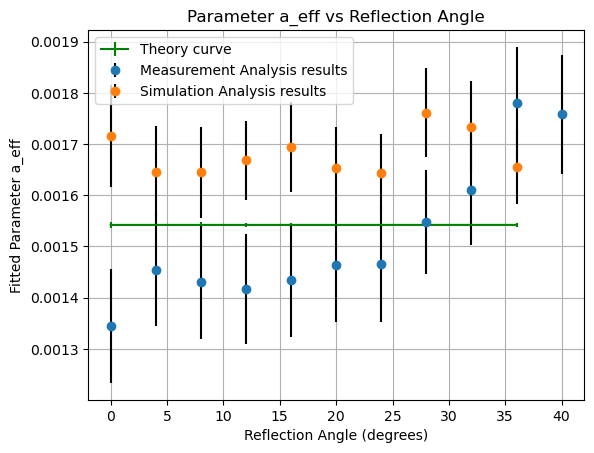
\includegraphics[width=0.7\linewidth]{graphs/a_eff_errorbar.png}
    \caption{Estimation of the inverse attenuation length parameter, the $a_{eff}$, with respect to the reflection angle by all means possible in this lab course}
    \label{a_eff}
\end{figure}

We have a peculiar result, the theory curve sits almost flat in between the two data distributions that seem to be mirroring each other by the axis of the theory curve between [0,25] degrees angle. Although, the general values are in the same ballpark with the added errorbar.